
\newpage
\null
\thispagestyle{empty}
\newpage
\addcontentsline{toc}{chapter}{Obadiah}
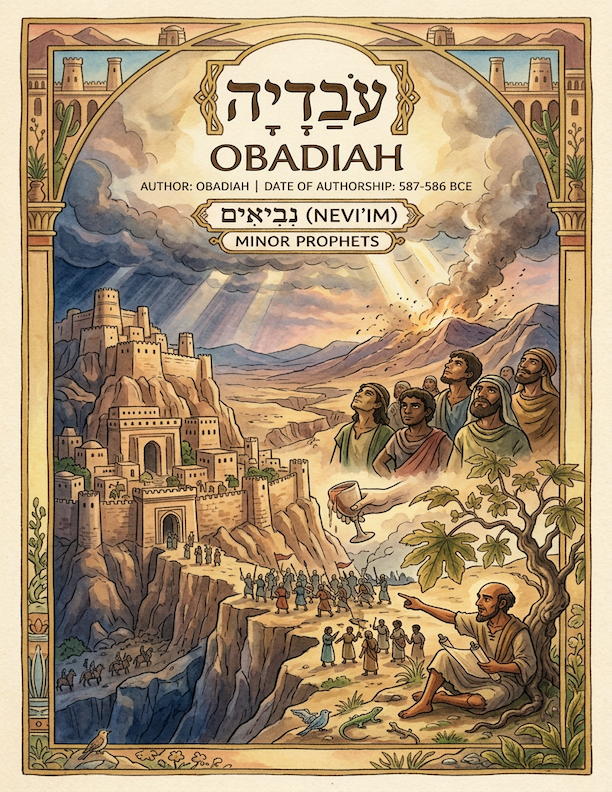
\includepdf[pages=1, fitpaper=false, width=\paperwidth, height=\paperheight, , keepaspectratio=false]{images/divider2/obadiah_2.png}
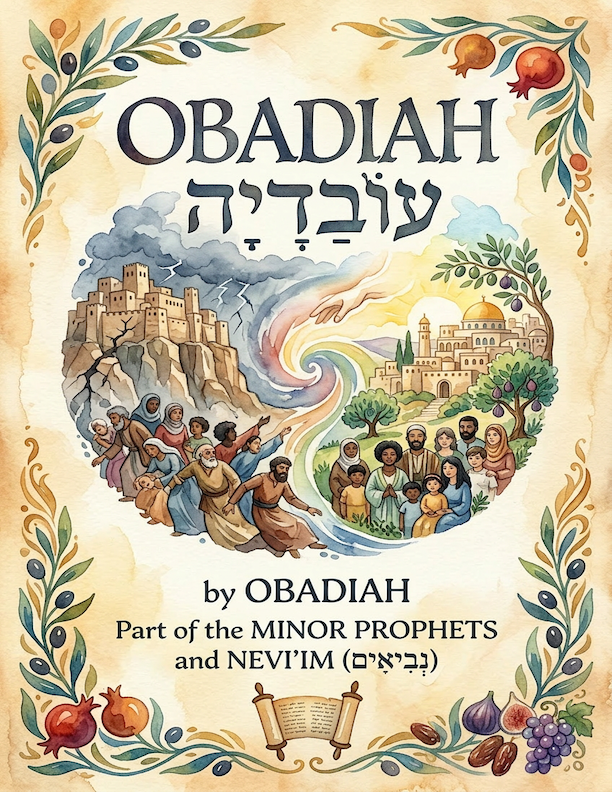
\includepdf[pages=1, fitpaper=false, width=\paperwidth, height=\paperheight, , keepaspectratio=false]{images/divider1/obadiah.png}

\includepdf[pages=1, fitpaper=false, width=\paperwidth, height=\paperheight, , keepaspectratio=false]{images/8.5x11-Dot-Grid.png}

\includepdf[pages=1, fitpaper=false, width=\paperwidth, height=\paperheight, , keepaspectratio=false]{images/8.5x11-Dot-Grid.png}
\mybook{Obadiah}
\vspace{-1.36in}

\mychapter{}
\myverse*{}The vision of Obadiah. This is what the Lord\footnote{1:1 The word translated “Lord” (mixed case) is “Adonai.”} GOD\footnote{1:1 When rendered in ALL CAPITAL LETTERS, “LORD” or “GOD” is the translation of God’s Proper Name.} says about Edom. We have heard news from the LORD, and an ambassador is sent among the nations, saying, “Arise, and let’s rise up against her in battle. \myverse{}Behold,\footnote{1:2 “Behold”, from “הִנֵּה”, means look at, take notice, observe, see, or gaze at. It is often used as an interjection.} I have made you small among the nations. You are greatly despised. \myverse{}The pride of your heart has deceived you, you who dwell in the clefts of the rock, whose habitation is high, who says in his heart, ‘Who will bring me down to the ground?’ \myverse{}Though you mount on high as the eagle, and though your nest is set among the stars, I will bring you down from there,” says the LORD. \myverse{}“If thieves came to you, if robbers by night—oh, what disaster awaits you—wouldn’t they only steal until they had enough? If grape pickers came to you, wouldn’t they leave some gleaning grapes? \myverse{}How Esau will be ransacked! How his hidden treasures are sought out! \myverse{}All the men of your alliance have brought you on your way, even to the border. The men who were at peace with you have deceived you, and prevailed against you. Friends who eat your bread lay a snare under you. There is no understanding in him.”

\myverse{}“Won’t I in that day”, says the LORD, “destroy the wise men out of Edom, and understanding out of the mountain of Esau? \myverse{}Your mighty men, Teman, will be dismayed, to the end that everyone may be cut off from the mountain of Esau by slaughter. \myverse{}For the violence done to your brother Jacob, shame will cover you, and you will be cut off forever. \myverse{}In the day that you stood on the other side, in the day that strangers carried away his substance and foreigners entered into his gates and cast lots for Jerusalem, even you were like one of them. \myverse{}But don’t look down on your brother in the day of his disaster, and don’t rejoice over the children of Judah in the day of their destruction. Don’t speak proudly in the day of distress. \myverse{}Don’t enter into the gate of my people in the day of their calamity. Don’t look down on their affliction in the day of their calamity, neither seize their wealth on the day of their calamity. \myverse{}Don’t stand in the crossroads to cut off those of his who escape. Don’t deliver up those of his who remain in the day of distress. \myverse{}For the day of the LORD is near all the nations! As you have done, it will be done to you. Your deeds will return upon your own head. \myverse{}For as you have drunk on my holy mountain, so all the nations will drink continually. Yes, they will drink, swallow down, and will be as though they had not been. \myverse{}But in Mount Zion, there will be those who escape, and it will be holy. The house of Jacob will possess their possessions. \myverse{}The house of Jacob will be a fire, the house of Joseph a flame, and the house of Esau for stubble. They will burn among them and devour them. There will not be any remaining to the house of Esau.” Indeed, the LORD has spoken.

\myverse{}Those of the South will possess the mountain of Esau, and those of the lowland, the Philistines. They will possess the field of Ephraim, and the field of Samaria. Benjamin will possess Gilead. \myverse{}The captives of this army of the children of Israel, who are among the Canaanites, will possess even to Zarephath; and the captives of Jerusalem, who are in Sepharad, will possess the cities of the Negev. \myverse{}Saviors will go up on Mount Zion to judge the mountains of Esau, and the kingdom will be the LORD’s.